\usepackage{fontspec}
\setmainfont{texgyrepagella-regular.otf}[BoldFont=texgyrepagella-bold.otf,ItalicFont=texgyrepagella-italic.otf,BoldItalicFont=texgyrepagella-bolditalic.otf]
\setsansfont{texgyreheros-regular.otf}[BoldFont=texgyreheros-bold.otf,ItalicFont=texgyreheros-italic.otf]
\usepackage[french]{babel}
\usepackage[a4paper,margin=25mm,headheight=15pt,headsep=7mm,footskip=12mm]{geometry}
\usepackage{setspace}
\setstretch{1.14}
\usepackage[table]{xcolor}
\definecolor{Navy}{HTML}{193D5B}
\definecolor{Teal}{HTML}{257F79}
\definecolor{Purple}{HTML}{7659A6}
\definecolor{Orange}{HTML}{B96B24}
\definecolor{Red}{HTML}{BA3434}
\definecolor{Green}{HTML}{527A3F}
\definecolor{Light}{HTML}{F2F5F7}
\usepackage{graphicx,booktabs,longtable,array,tabularx}
\usepackage{caption,float,placeins,pdflscape}
\usepackage{enumitem,needspace,titlesec,fancyhdr}
\usepackage{tikz}
\usetikzlibrary{arrows.meta,positioning,calc,shapes.geometric}
\usepackage[most]{tcolorbox}
\usepackage{microtype,ifthen}
\usepackage{hyperref}
\hypersetup{colorlinks=true,linkcolor=Navy,citecolor=Navy,urlcolor=Teal,pdftitle={Rapport de stage - Architecture fonctionnelle Smart WMS},pdfauthor={FERHAN Abdelali},bookmarksnumbered=true}
\urlstyle{same}
\setlength{\parindent}{0pt}
\setlength{\parskip}{5pt plus 1pt}
\setlength{\emergencystretch}{2em}
\setlength{\LTpre}{8pt}
\setlength{\LTpost}{10pt}
\newlength{\TableWidth}
\newcolumntype{P}[1]{>{\raggedright\arraybackslash}p{#1}}
\renewcommand{\arraystretch}{1.15}
\setlist[itemize]{leftmargin=1.5em,itemsep=3pt,topsep=4pt}
\widowpenalty=10000
\clubpenalty=10000
\displaywidowpenalty=10000
\raggedbottom
\titleformat{\chapter}[display]{\sffamily\color{Navy}\bfseries\raggedright}{\normalsize\MakeUppercase{\chaptername}\ \thechapter}{8pt}{\LARGE}
\titlespacing*{\chapter}{0pt}{-8pt}{20pt}
\titleformat{\section}{\sffamily\large\bfseries\color{Navy}}{\thesection}{.6em}{}
\titlespacing*{\section}{0pt}{17pt}{7pt}
\captionsetup{font=small,labelfont=bf,justification=raggedright,singlelinecheck=false,skip=7pt}
\captionsetup[longtable]{position=top}
\renewcommand{\thefigure}{\ifnum\value{chapter}=0 I\else\thechapter\fi.\arabic{figure}}
\pagestyle{fancy}
\fancyhf{}
\fancyhead[L]{\sffamily\footnotesize\color{Navy}FERHAN Abdelali}
\fancyhead[R]{\sffamily\footnotesize\color{Navy}Rapport de stage | Smart WMS}
\fancyfoot[C]{\sffamily\small\thepage}
\renewcommand{\headrulewidth}{.3pt}
\fancypagestyle{plain}{\fancyhf{}\fancyfoot[C]{\sffamily\small\thepage}\renewcommand{\headrulewidth}{0pt}}
\newtcolorbox{problematique}{colback=Light,colframe=Navy,boxrule=.5pt,arc=0mm,title=Problématique directrice,fonttitle=\sffamily\bfseries,left=3mm,right=3mm,top=2mm,bottom=2mm}
\newcommand{\reportfigure}[2]{\begin{figure}[!htbp]\centering\ifthenelse{\equal{#1}{marche}}{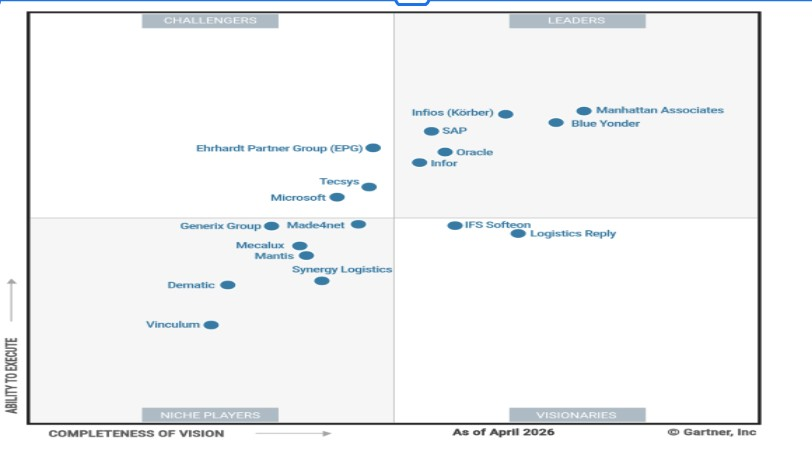
\includegraphics[width=.91\linewidth]{figures/revision/marche.png}}{\resizebox{\linewidth}{!}{\input{figures/revision/#1}}}\caption{#2}\label{fig:#1}\end{figure}\FloatBarrier}
\tikzset{flow/.style={-{Stealth[length=2.5mm]},draw=Navy,line width=.7pt},frame/.style={draw=Navy,line width=.6pt,fill=white},every node/.style={font=\sffamily\fontsize{10}{12}\selectfont,align=left,execute at begin node={\setlength{\parskip}{0pt}\raggedright}}}
% Fixed box geometry separates titles from body text in the detailed diagrams.
\newcommand{\pblock}[7]{%
  \draw[draw=#5!65,line width=.55pt,fill=white] (#1,#2) rectangle ++(#3,#4);
  \fill[#5!9] (#1,#2) rectangle ++(#3,.82);
  \node[anchor=north west,text width=\dimexpr #3cm-10pt\relax,inner sep=5pt,font=\sffamily\bfseries\fontsize{9.3}{11.8}\selectfont,text=#5] at (#1,#2) {#6};
  \node[anchor=north west,text width=\dimexpr #3cm-10pt\relax,inner sep=5pt,font=\sffamily\fontsize{9}{11.5}\selectfont] at (#1,{#2+.87}) {#7};
}
\newcommand{\pband}[3]{\node[anchor=west,text=#3,font=\sffamily\bfseries\fontsize{11}{13}\selectfont,inner sep=0pt] at (0,#1) {#2};}
\newcommand{\fblock}[7]{
  \draw[draw=#5,line width=.6pt,fill=white] (#1,#2) rectangle ++(#3,#4);
  \fill[#5!10] (#1,#2) rectangle ++(#3,1.15);
  \node[anchor=north west,text width=\dimexpr #3cm-8pt\relax,inner sep=4pt,font=\sffamily\bfseries\fontsize{9}{11}\selectfont,text=#5] at (#1,#2) {\ifthenelse{\equal{#5}{Red}}{\color{Navy}}{}#6};
  \node[anchor=north west,text width=\dimexpr #3cm-8pt\relax,inner sep=4pt,font=\sffamily\fontsize{9}{11.5}\selectfont] at (#1,{#2+1.2}) {#7};
}
